\paragraph{QuizziPedia::Front-End::ModelViews::StatisticsModelView}

\label{QuizziPedia::Front-End::ModelViews::StatisticsModelView}

\begin{figure}[ht]
	\centering
	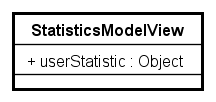
\includegraphics[scale=0.5,keepaspectratio]{UML/Classi/Front-End/QuizziPedia_Front-end_ModelView_StatisticsModelView.png}
	\caption{QuizziPedia::Front-End::ModelViews::StatisticsModelView}
\end{figure} \FloatBarrier

\begin{itemize}
	\item \textbf{Descrizione}: classe di tipo modelview la cui istanziazione è contenuta all'interno della variabile di ambiente \texttt{\$scope} di \textit{Angular\ped{G}}. All'interno di essa sono presenti le variabili e i metodi necessari per il \textit{Two-Way Data-Binding\ped{G}} tra la \textit{view\ped{G}} \texttt{UserView} e il \textit{controller\ped{G}} \texttt{StatisticsController};
	\item \textbf{Utilizzo}: viene utilizzata per effettuare il \textit{Two-Way Data-Binding\ped{G}} tra la \textit{view\ped{G}} \texttt{UserView} e il \textit{controller\ped{G}} \texttt{StatisticsController} rendendo disponibili variabili e metodi;
	\item \textbf{Relazioni con altre classi}: 
	\begin{itemize}
		\item \textbf{OUT \texttt{UserView}}: \textit{view\ped{G}} contenente le direttive dei dati personali dell'utente, delle sue statistiche relative ai questionari e agli allenamenti effettuati e dei questionari a cui è iscritto; 
		\item \textbf{OUT \texttt{StatisticsController}}: questa classe permette di le statistiche di un utente.
	\end{itemize}
	\item \textbf{Attributi}: 
	\begin{itemize}
		\item \texttt{+ userStatistic: Object} \\ Oggetto contenente le statistiche di un utente.
	\end{itemize}
\end{itemize}	

